\section{Appendix}
\begin{figure}[H]
    \captionsetup{format=plain}
    \makebox[\textwidth]{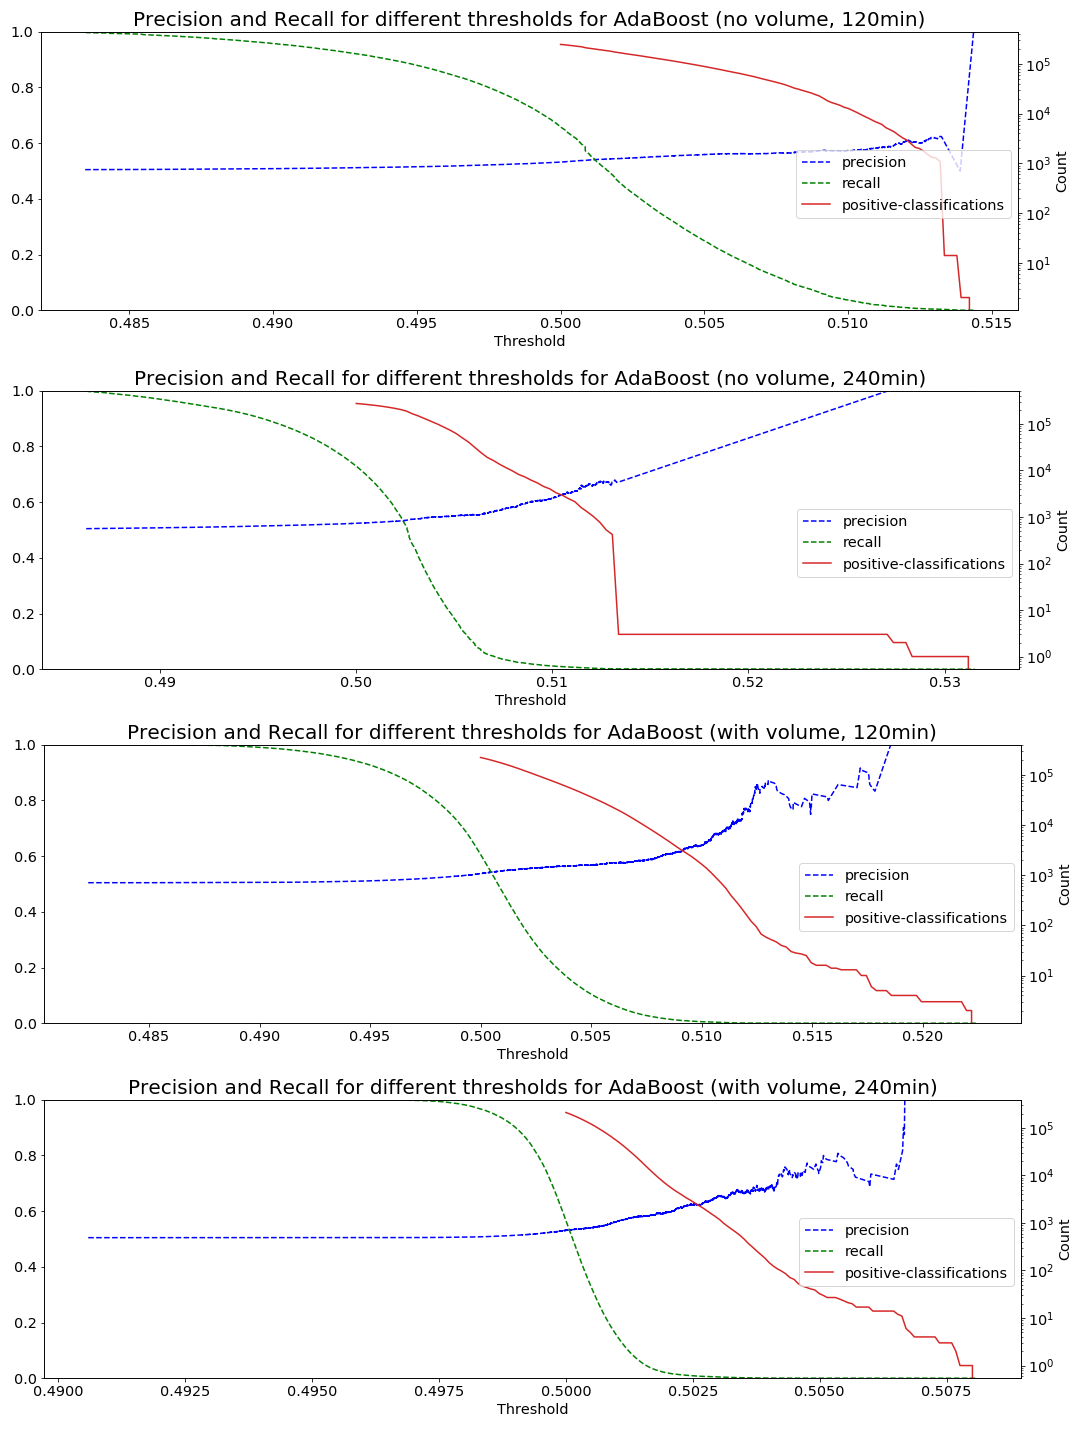
\includegraphics[width=165mm]{adaboost/adaboost_threshold_vs_precision.png} }
    \caption{ 
            This figure illustrates the precision, recall and up-classifications of the 
            AdaBoost for different thresholds and specifications.
        }
    \label{fig:adaboost_threshold_vs_precision}
\end{figure}

\begin{figure}[H]
    \captionsetup{format=plain}
    \makebox[\textwidth]{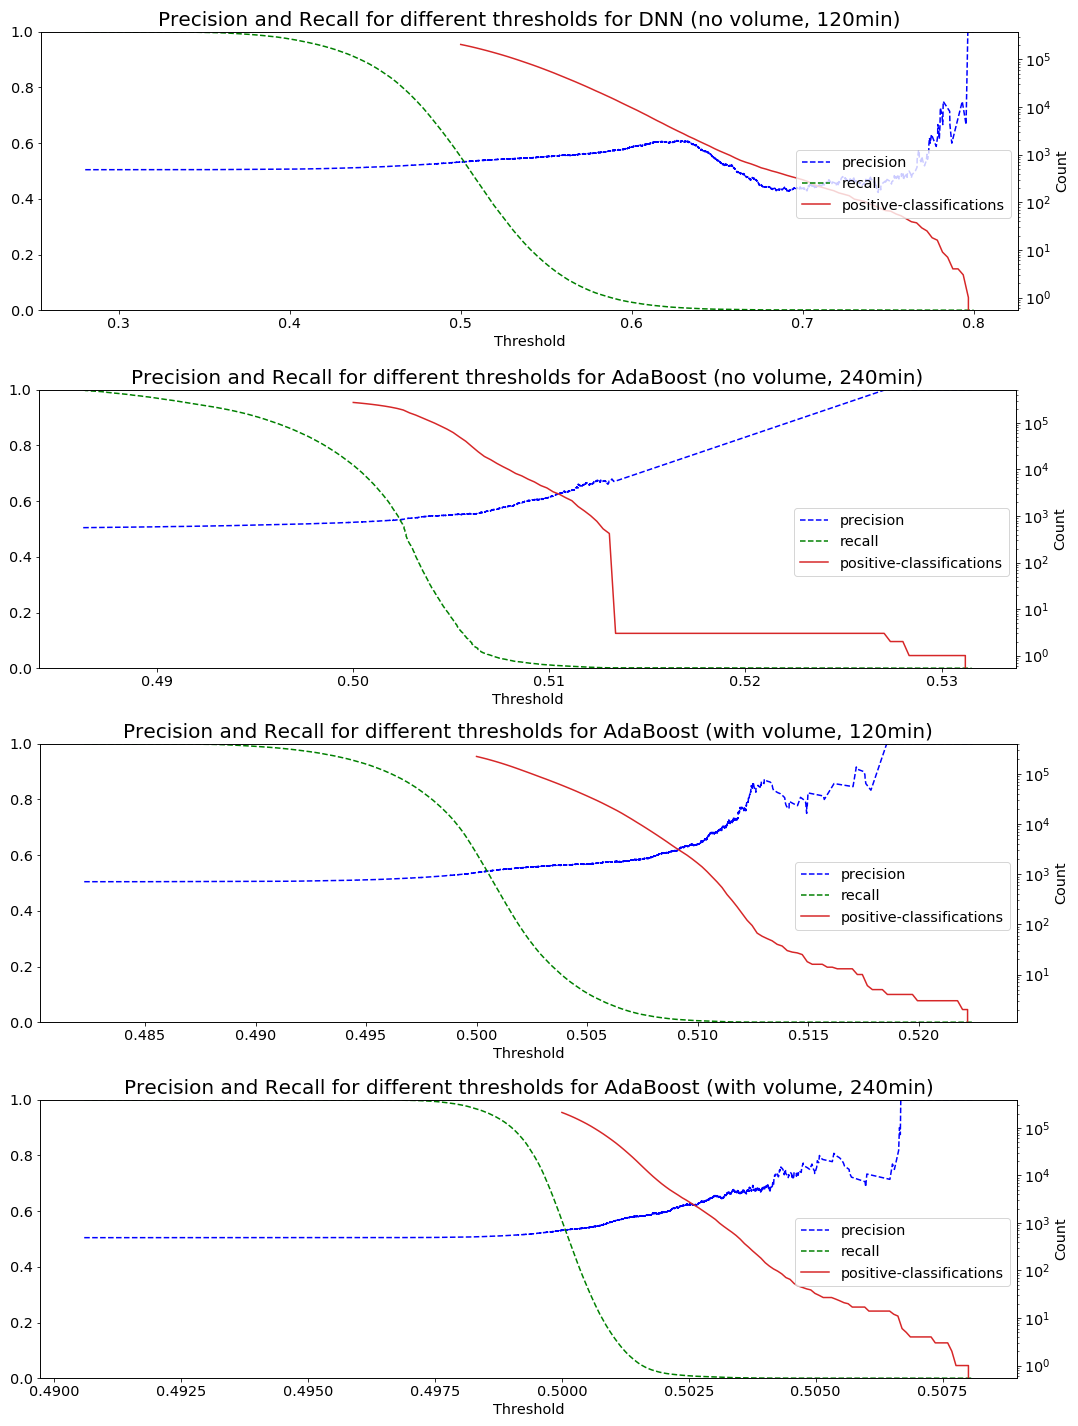
\includegraphics[width=165mm]{ann/ann_threshold_vs_precision.png} }
    \caption{ 
            This figure illustrates the precision, recall and up-classifications of the Deep Neural Network for different thresholds
            and specifications.
        }
    \label{fig:ann_threshold_vs_precision}
\end{figure}

\begin{figure}[H]
    \captionsetup{format=plain}
    \makebox[\textwidth]{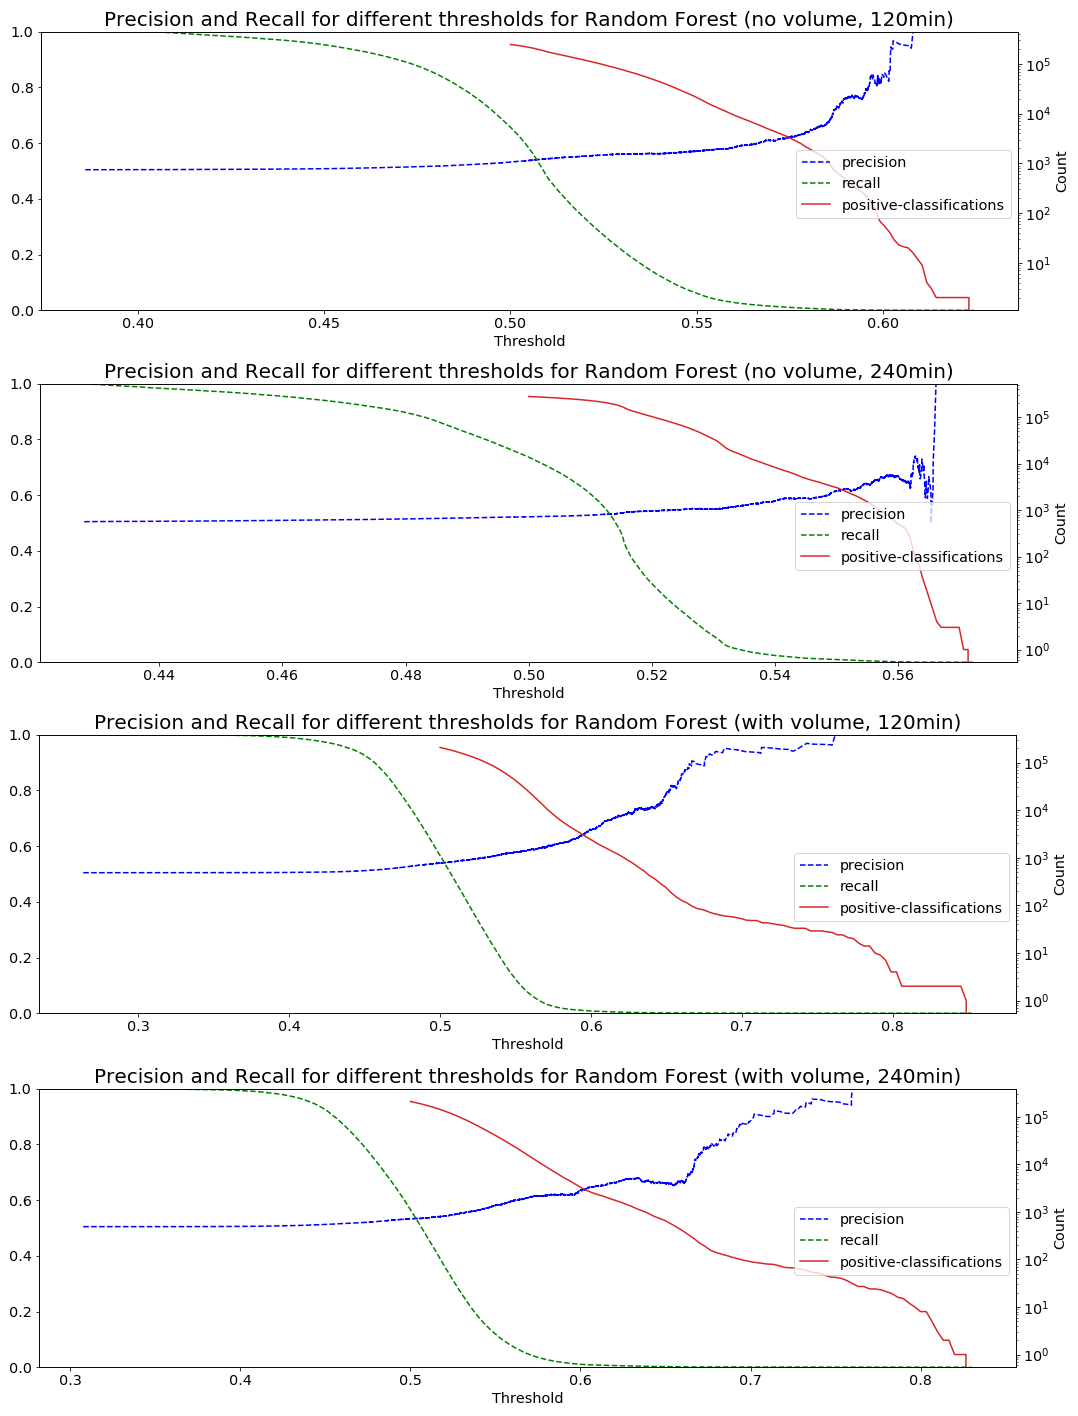
\includegraphics[width=165mm]{forest/forest_threshold_vs_precision.png} }
    \caption{ 
            This figure illustrates the precision, recall and up-classifications of the Random Forest for different thresholds
            and specifications.
        }
    \label{fig:forest_threshold_vs_precision}
\end{figure}

\begin{figure}[H]
    \captionsetup{format=plain}
    \makebox[\textwidth]{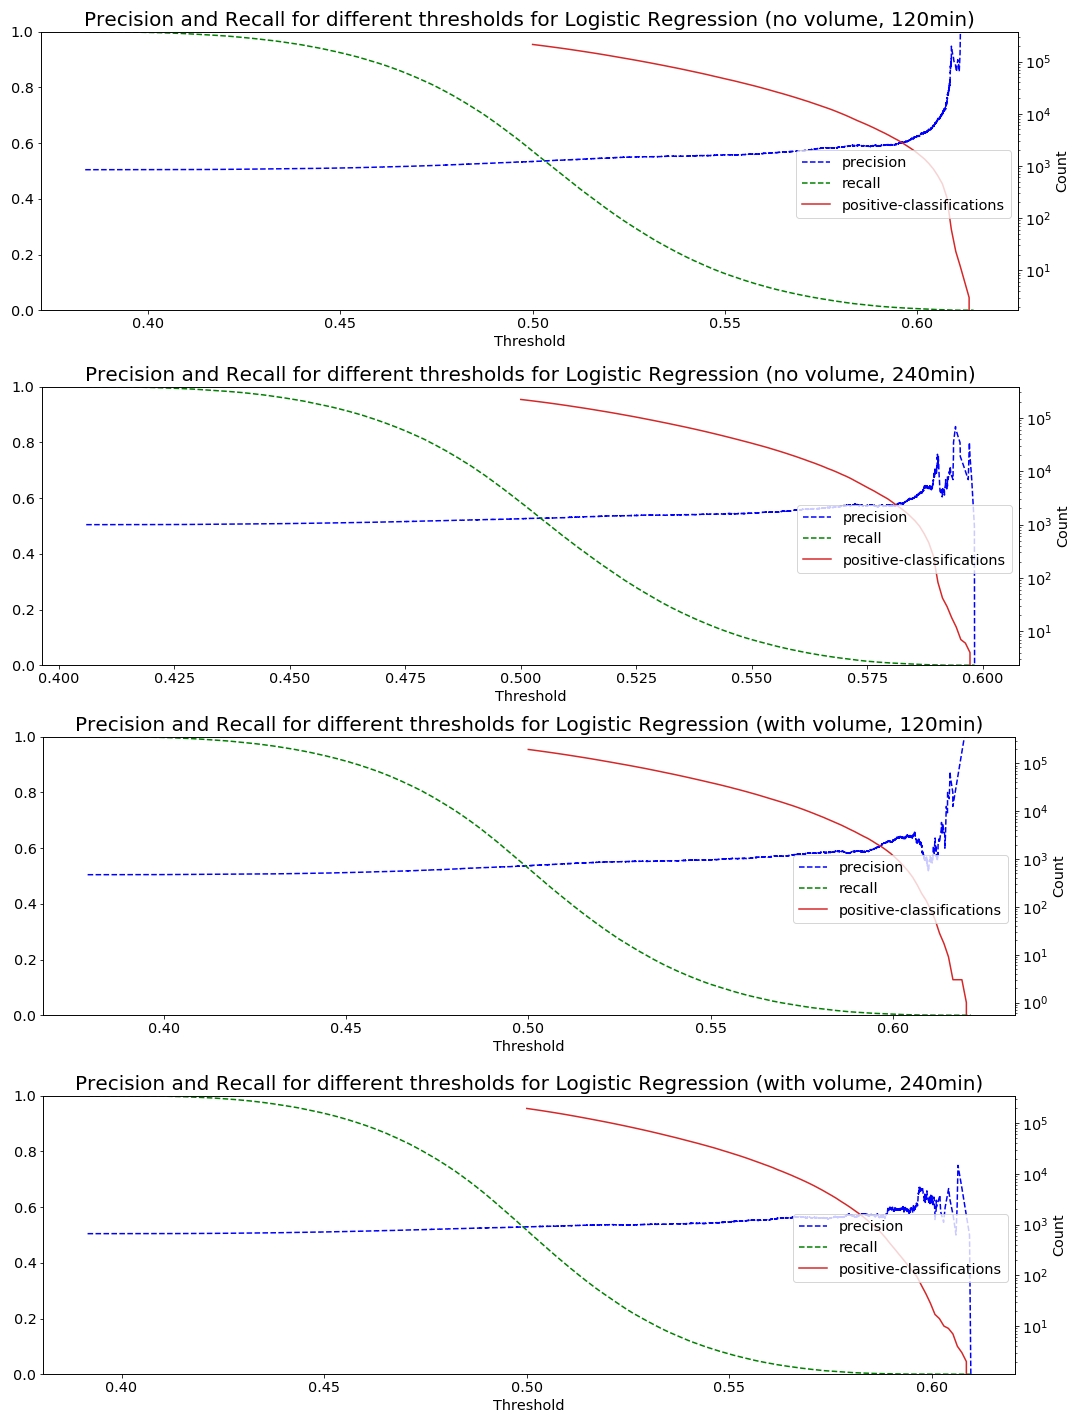
\includegraphics[width=165mm]{logistic/logistic_threshold_vs_precision.png} }
    \caption{ 
            This figure illustrates the precision, recall and up-classifications of the Logistic Regression for different thresholds
            and specifications.
        }
    \label{fig:logistic_threshold_vs_precision}
\end{figure}


\begin{figure}[H]
    \captionsetup{format=plain}
    \makebox[\textwidth]{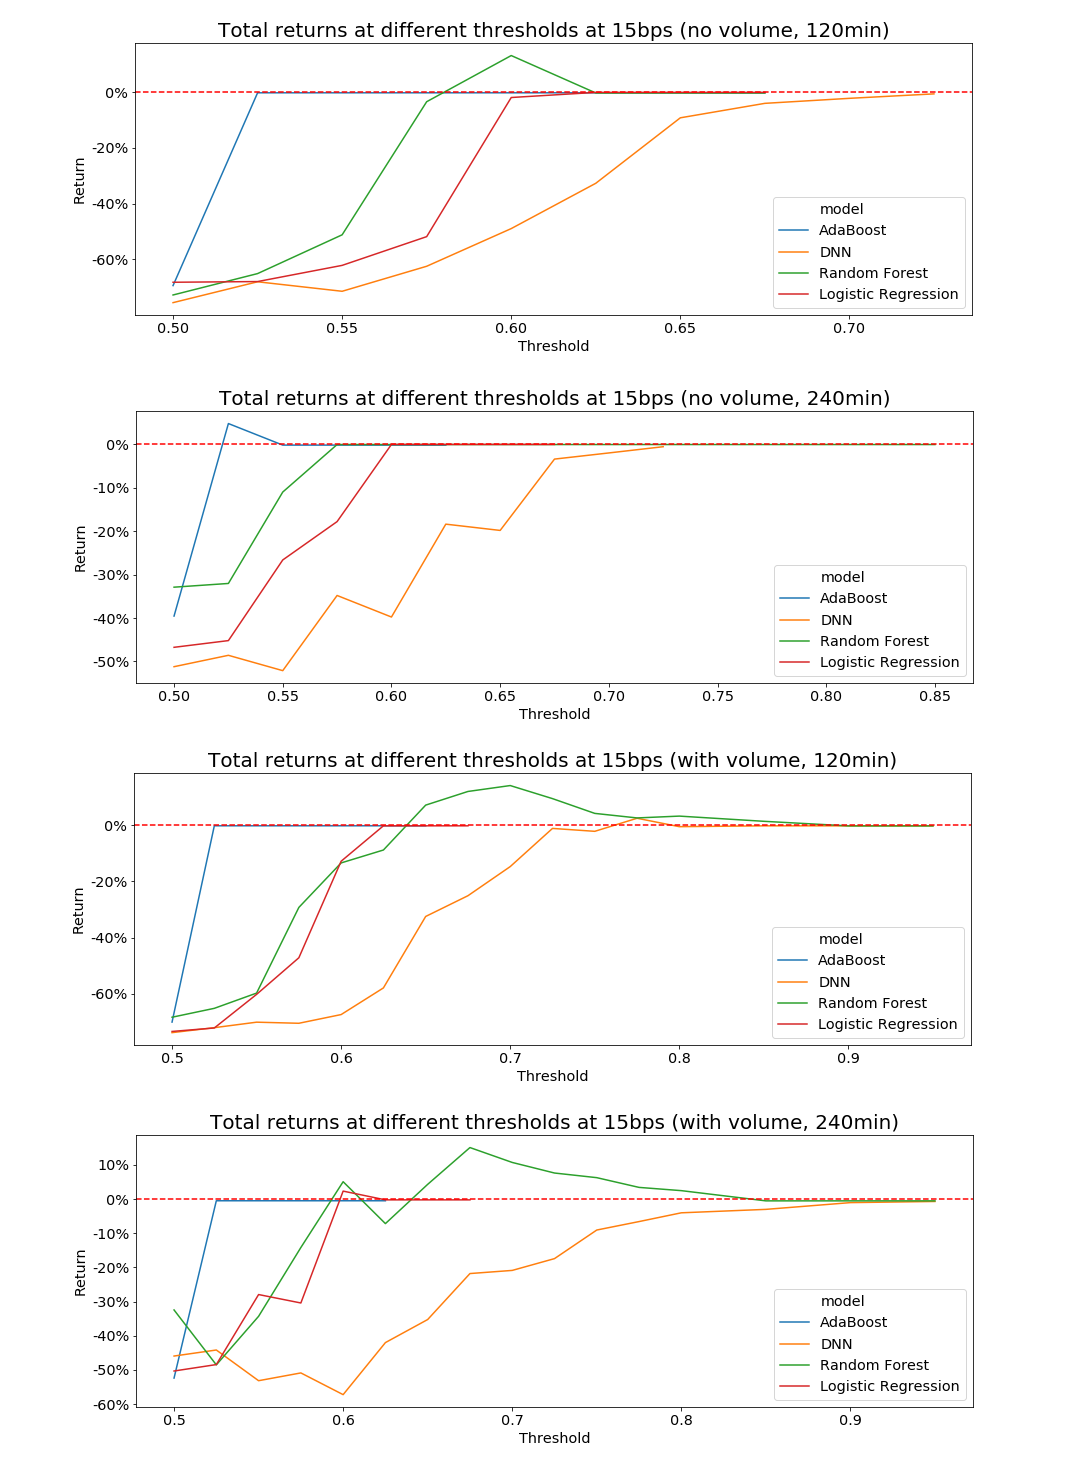
\includegraphics[width=165mm]{all/all_threshold_vs_return.png} }
    \caption{ 
        This figure illustrates total returns at a transaction cost of 15bps over the trading period for different thresholds
        and specifications.
        }
    \label{fig:all_threshold_vs_return}
\end{figure}


\begin{figure}[H]
    \captionsetup{format=plain}
    \makebox[\textwidth]{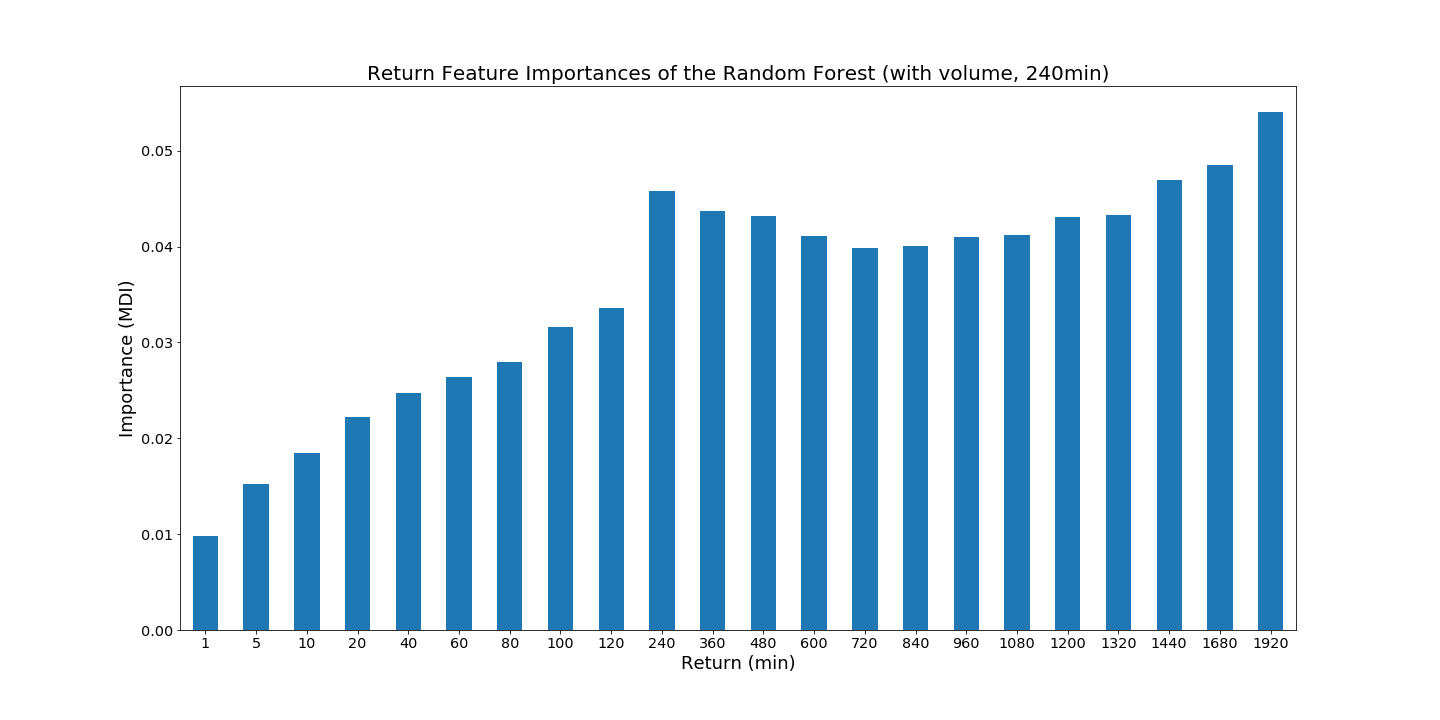
\includegraphics[width=165mm]{forest/forest_return_feature_importance_with_volume_future_2state_movement_240min.png} }
    \caption{ 
            This figure illustrates the feature importances of the Random Forest according to MDI \cite{louppe2015variableImportance}
            for different return deltas in minutes as described in chapter \ref{ch:training_trading}. 
            The Random Forest was trained on features containing both returns and volumes and a forecast duration of 240min.
        }
    \label{fig:forest_return_feature_importance_with_volume_240min}
\end{figure}

\begin{figure}[H]
    \captionsetup{format=plain}
    \makebox[\textwidth]{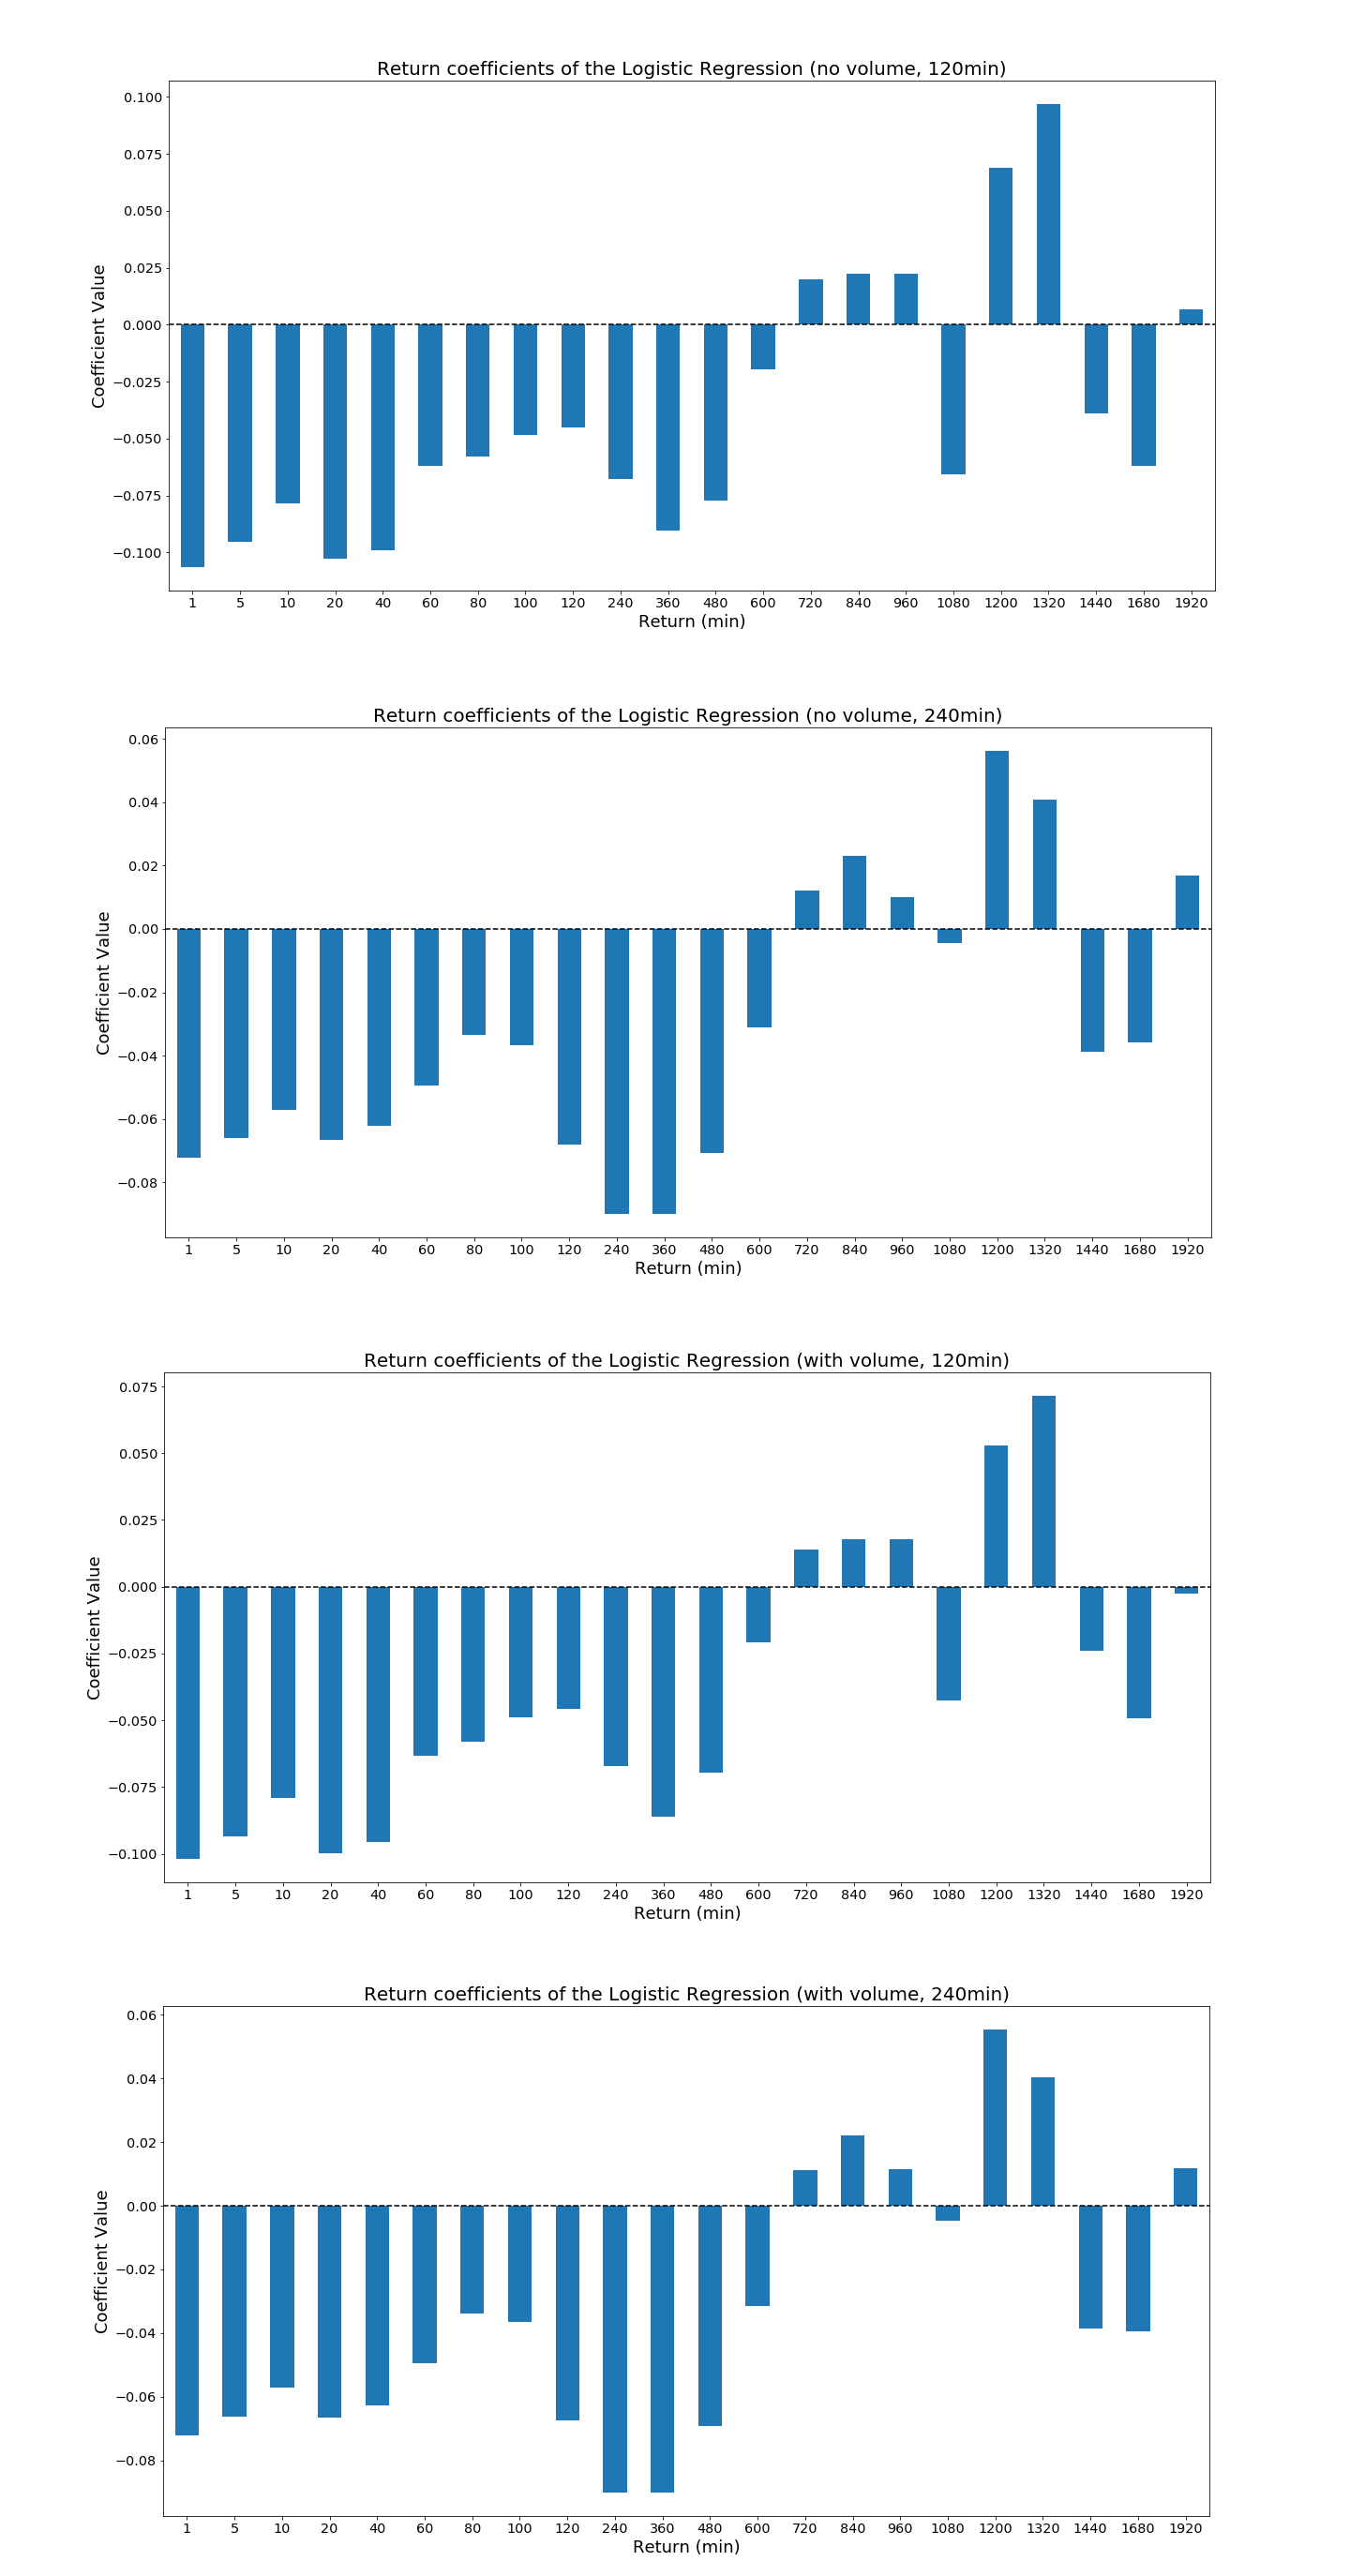
\includegraphics[width=125mm]{logistic/logistic_return_coefficients.png} }
    \caption{ 
            This figure illustrates the coefficients of returns estimated by the Logistic Regression
            for different time periods in minutes for different feature and target specification.
        }
    \label{fig:logistic_return_coefficients}
\end{figure}

\pagebreak
